\newpage
\section{Aufbau der App}

%--------------------------------------------------------------------------------------------
\subsection{Klassendiagramm} \index{Klassendiagramm}

\begin{figure}[h!]
\label{fig:class_diagramm_activity}
\centering
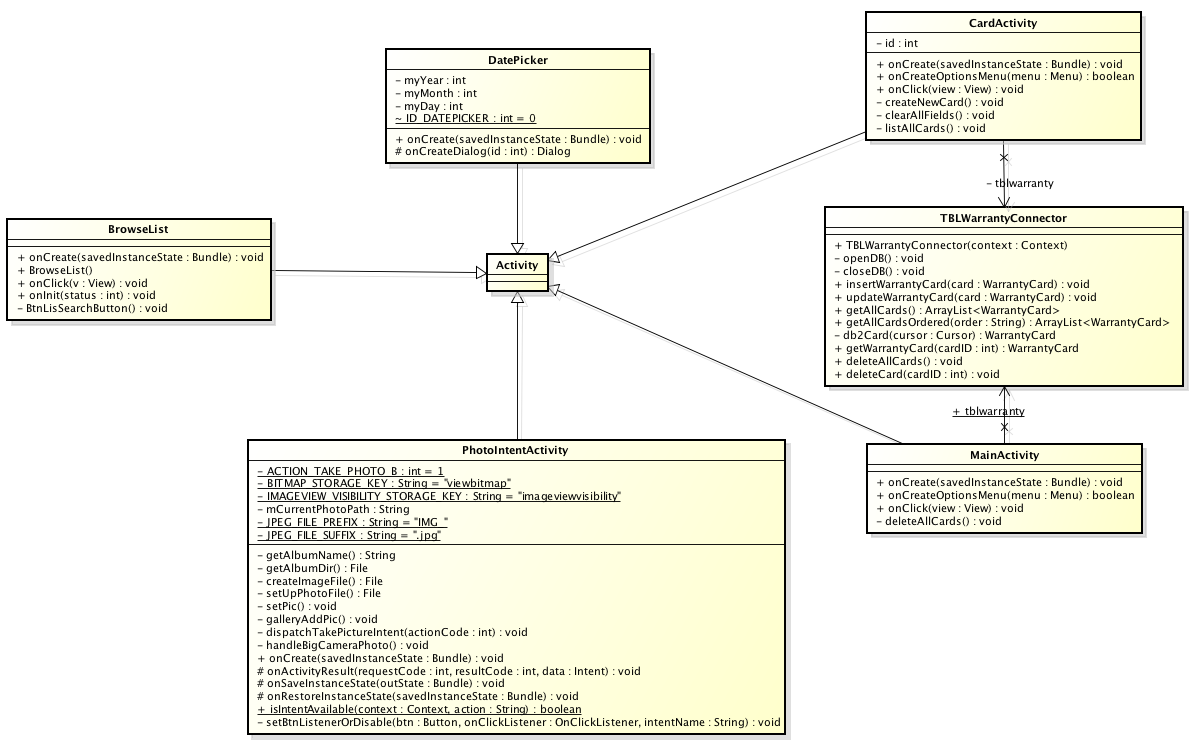
\includegraphics[width=\textwidth]{class_diagramm_activity.png} 
\caption{Klassendiagramm Activity}
\end{figure}



\textcolor{red}{!!!! HIER KOMMEN NOCH MEHR DIAGRAMME !!!!} \\ \\ \\ \\

\textcolor{red}{!!!! KOMMT HIER NOCH TEXT? !!!!}





%--------------------------------------------------------------------------------------------
\subsection{Permissions} \index{Permissions}
Die Warranty App ben�tigt wenige zus�tzliche Rechte. Um Bilder speichern zu k�nnen ist jedoch ein Speicherplatz erforderlich. Da die meisten Android basierten Smartphones einen sehr kleinen internen Speicher haben, bietet sich der externe Speicher bestens an. Je nach Modell ist dies entweder eine zus�tzlichen MicroSD [Glossar] Karte oder einfach eine zus�tzliche logische Partition auf dem internen Speicher. Der Vorteil dieses externen Speichers ist, dass man ihn ohne weiteres auf dem Computer einh�ngen und auf die Dateien zugreifen kann.

Um auf diesen externen Speicher zuzugreifen, wird folgende Zeile im Manifest.xml ben�tigt.
\lstset{language=Java, numbers=left}


\begin{lstlisting}[label=lst:latex.listing,captionpos=b, caption=Android permission for external Storage]
<uses-permission android:name="android.permission.WRITE_EXTERNAL_STORAGE" />
\end{lstlisting}

Nebst dem Zugriff auf den Speicher, bedient sich Warranty den Kamerafunktionalit�ten. Da diese ebenfalls explizit erlaubt werden m�ssen, wird das entsprechende Recht im Manifest.xml hinterlegt.
\lstset{language=Java, numbers=left}
\begin{lstlisting}[label=lst:latex.listing,captionpos=b, caption=Android permission for Camera]
<uses-permission android:name="android.permission.CAMERA" />
\end{lstlisting}


%--------------------------------------------------------------------------------------------
\newpage
\subsection{Datenbank} \index{Datenbank} \index{DBMS}
Auch wenn wir auf unserem Smartphone eine Datenbank ben�tigen, so scheint die Idee, ein vollumf�ngliches \abkDef{DBMS}{\textbf{D}atabase \textbf{M}anagement \textbf{S}ystem}  wie beispielsweise MySQL oder PostgreSQL zu installieren absurd. Zum einen ben�tigen wir Features wie ein Client/Server Model, Partitioning oder ein ausgefeiltes Zugriffsberechtigungssystem nicht, zum anderen steht die dazu ben�tigte Performance auf einem Smartphone schlicht und einfach nicht zur Verf�gung. 
\newline
Um dennoch eine Datenbank auf einem Smartphone verwenden zu k�nnen, bietet sich SQLite an. SQLite ist eine Programmbibliothek, die sich direkt in der Applikation einbinden l�sst und somit keinen Server- Prozess ben�tigt, also ressourcensparend ist. Die gesamte Datenbank inklusive aller Tabellen, Indizes und Werten werden in einer einzigen Datei abgelegt, was ein paralleles Schreiben auf die Datenbank unm�glich macht.
\newline
Dank der nativen SQLite Unterst�tzung von Android, f�llt ein aufw�ndiges einbinden einer 3rd Party Library weg.
\\
